%&latex
\documentclass[a4paper]{report}
\usepackage{commons/commons}
\usepackage{commons/note_style}
\usepackage{commons/code_style}
\usepackage[normalem]{ulem}
\usepackage{comment}
\usepackage{titlesec}
\titleformat{\chapter}[display]
  {\normalfont\sffamily\big\bfseries\color{black}}
  {\chaptertitlename\ \thechapter}{5pt}{\huge}
%\excludecomment{figure}
\usepackage{amsbsy}
\usepackage{amstext}

\graphicspath{{./fig/}}
\begin{document}

%+Title
\title{Machine Learning Quicksheet}
\author{Daniel D. Zhang}
\date{Winter 2015. \today}
\maketitle
%-Title

%+Abstract
%\begin{abstract}
%This is the notes for CSE 232A.
%\end{abstract}
%-Abstract

%+Contents
\tableofcontents
%-Contents
\chapter*{Preface}
\section*{Acronyms}
\begin{obeylines}
\rih{distr}. Distribution
\rih{Pr}. Probability
\end{obeylines}
\chapter{Introduction}
Mapping
$$
f: \mat{X} \ra \mat{Y}. 
$$
Outline 
\begin{enumerate}
\item Nonparametric methods
\begin{enumerate}
\item NN (nearest neighbor)
\item Decision tree 

$\ra$ benefits: 1) unbounded input size; 2) arbitrary complex model
\end{enumerate}
\item Classification with parameterized models 

General ways to classify 
\begin{enumerate}
\item Generative, generative probability - Bayes, Fisher 
\item Discriminative, boundary - SVM, logistic regression 
\end{enumerate}
\item Combining classifiers 
\item Representation learning 
\end{enumerate}

\chapter{Nearest Neighbor}
\section{kNN}
\subsection{Parameter Selection $k$}
\begin{enumerate}
\item Hold-out set. Choose a subset $V\subset S$ as a validation set 
$$
k = \arg\min_k \sum_{(x, y)\in V} \textbf{1}(\Gamma_k(S\backslash V, x)\neq y)
$$
\item Leave-one-out cross-validation 
$$
k = \arg\min_k \sum_{(x, y)\in S} \textbf{1}(\Gamma_k(S\backslash\{(x, y)\}, x)\neq y)
$$
\end{enumerate}
\subsection{Distance function}
\subsubsection{$l_p$ norms}

\subsubsection{Metric space} 
distance function $d: \mat{X}\times\mat{X}\ra \R$ is a metric iff:
\begin{enumerate}
\item $\geq0$
\item $=0$ iff equal
\item symmetry
\item triangle inequality
\end{enumerate}

\section{Statistical Learning Theory}
\begin{enumerate}
\item distribution over $x$, pdf: $\mu(x)$
\item distribution over $P(y=1|x)$: $\eta(x)$
\item classification rule $h: \mat{X}\ra\{0, 1\}$
\item bayes risk (general form): $R(h)=Pr\big(h(X)\neq Y\big)$
\begin{align*}
R(h) &= \E_x Pr\big(h(x)\neq y)\big) \\
&= \int pdf(x)\cdot Pr\big(h(x)\neq y)\big) \diff x
\end{align*}
\item Binary bayes-optimal classifier
\begin{eqnarray*}
h^*(x) = \left\{ \begin{array}{rl}
  1 &\mbox{ if }\eta(x)>\frac{1}{2}\\
  0 &\mbox{ ow}
       \end{array} \right.       
\end{eqnarray*}
with mim risk:
\begin{align*}
R(h^*) &= \E_x \min\Big(\eta(X), 1-\eta(X)\Big) \\
&= \int pdf(x)\cdot \min\Big(\eta(X), 1-\eta(X)\Big) \diff x
\end{align*}


\end{enumerate}





\chapter{Decision Tree}
\section{Construction}
Greedy algorithm to split one of $\{leaves\}$ s.t. most decrease the uncertainty in tree. \subsection{Uncertainty measure}
\begin{enumerate}
\item Misclassification rate: $1-\max_i p_i$
\item Gini index: $\sum_{i\neq j} p_i p_j$
\item Entropy: $\sum_i p_i \log\frac{1}{p_i}$
\end{enumerate}
Reduction in uncertainty measure $u(\cdot)$.
$\Big(u(S)-(p_Lu(S_L)+p_Ru(S_R))\Big)|S|$
\subsection{Overfitting \& Pruning}
\begin{enumerate}
\item Training error 
$$\hat\varepsilon(h) = \frac{1}{n}\sum_i \textbf{1}\Big(h(X^{(i)})\neq Y^{(i)}\Big)$$
\item True error, underlying error 
$$\varepsilon(h)=Pr_{(x,y)\sim D}\Big(h(x)\neq y \Big)$$
, where $D$ is the underlying distribution. 
\item Validation error, as an indicator for true error. Validation set $V$. 
$$\varepsilon(h,V) = \frac{1}{|V|}\sum_{(x, y)\in V} \textbf{1}\Big(h(x)\neq y\Big)$$
If $V$ is chosen iid from $D$, then: 
\begin{align*}
\E[\varepsilon(h, V)] &=\varepsilon(h)\\
\operatorname{Var}[\varepsilon(h, V)] &= \frac{1}{|V|}
\end{align*}
\end{enumerate}


\chapter{Generative Model}
\section{Bayes Generative Model}
\subsection{General}
Underlying distribution $D$ over $\mat{X}\times \mat{Y}$

The overall density is a mixture of the individual densities,
$$
Pr(x) = \sum_i \pi_i P_i(x)
$$

Then bayes predictions:
$$
Pr(y=j|x) = \frac{Pr(y=j)Pr(x|y=j)}{Pr(x)} = \frac{\pi_jP_j(x)}{\sum_i \pi_i P_i(x)}
$$
, where $\pi_j=Pr(y=j), P_j(x)=Pr(x|y=j)$, $y$ here is for one data point. 

Notation-wise, $i$ is for data point index, $j$ is for class label index, $d$ for dim index.
\subsection{Model $P_i(x)$}
\subsubsection{Naive Bayes}
Assume indpt among the dimension:
\begin{align*}
P_j(x) &= \prod_d P_{jd}(x_d) \\
P_{jd}(x_d) &= Pr(x_d|y=j) 
\end{align*}
For binary input $\mat{X}=\{0, 1\}^p$
\begin{align*}
p_{jd} &= Pr(x_d=1|y=j)\\
\hat p_{jd} &= \frac{n_{jd}}{n_{j}} \text{ by ML}\\
\hat p_{jd} &= \frac{n_{jd}+\alpha}{n_{j}+D\alpha} \text{ smoothing, where } d= 0,...,D-1
\end{align*}
Binary-class classification, in \textit{power selection} notation:
$$
\hat y = \arg\max_j \quad \pi_j \prod_d p_{jd}^{x_d}(1-p_{jd})^{(1-x_d)}
$$
\subsubsection{Multinomial naive Bayes}
The example of application of multinomial naive Bayes is for document data. 

Ignore the order of dimension (\textbf{bag of words}); each dimension can take multiple values.

Per value over value set $V$ per toplic:
$$
p = (p_1,..., p_{|V|})
$$
, where $\forall i, p_i\geq 0, \sum_i p_i=1$.

For input data $x=(x_1, ..., x_{|V|})$, where $x_i$ means count of value $V_i$ (term frequency), for each topic $j$:
\begin{align*}
Pr_j(x) = \prod_{i=1}^{|V|}p_{ji}^{x_i}
\end{align*}
Then the classification rule is: 
$$
\hat y = \arg \max_j\quad \pi_j \prod_{i=1}^{|V|}p_{ji}^{x_i}
$$

In verbose mathematical expression:
\begin{align*}
P(y|x)\propto P(x|y)P(y)&=P(y)\prod_{d=1}^{D}P(v_d|y)^{|c_d|}\\
&=P(y)\prod_{i=1}^{N}P(x_i|y)
\end{align*}
\section{Gaussian}
\subsection{Basics}
\begin{align*}
& var(X) = \E(X-\mu)^2 = \E(X^2)-\mu^2 \\
& cov(X, Y) = \E[(X-\mu_X)(Y-\mu_Y)] = \E[XY]-\mu_X\mu_Y \\
& corr(X, Y) = \frac{cov(X, Y)}{\sigma(X)\sigma(Y)}
\end{align*}


\subsection{Multivariate Gaussian}
\subsubsection{Bivariate}
\begin{align*}
\mu &= [\mu_X, \mu_Y]^T \\
\Sigma &= \begin{bmatrix}
\Sigma_{XX} & \Sigma_{XY} \\
\Sigma_{YX} & \Sigma_{YY} 
\end{bmatrix}\\
&= \begin{bmatrix}
\operatorname{var}(X) & \operatorname{cov}(X,Y) \\
\operatorname{cov}(X,Y) & \operatorname{var}(Y)
\end{bmatrix}
\end{align*}
, the the values in $\Sigma$ can describe the shape of the bivariate gaussian distribution.


\subsubsection{Multivariate}
pdf:
$$
p(x) = \frac{1}{\sqrt{(2\pi)^p|\Sigma|}}\exp\Big(-\frac{1}{2}(\vec x-\vec\mu)^T\Sigma^{-1}(\vec x-\vec\mu)\Big)
$$
, where $\vec\mu=\E \vec x, \Sigma=\E(\vec x-\vec\mu)(\vec x-\vec\mu)^T=(X-\vec\mu)(X-\vec\mu)^T$. Algebraically, $\Sigma_{ij}=\operatorname{cov}(X_i, X_j)$. 

The $(\vec x-\vec\mu)^T\Sigma^{-1}(\vec x-\vec\mu)$ can be rewrite as: 
$$
(\vec x-\vec\mu)^T\Sigma^{-1}(\vec x-\vec\mu) = \sum_{i, j} \Sigma^{-1}_{ij} (\vec x_i-\vec \mu_i)(\vec x_j-\vec \mu_j)
$$

\subsubsection{Classification}
\begin{align*}
\pi_1 P_1(x) > \pi_2 P_2(x) &\equiv x^T Mx+2w^Tx \geq \theta \\
&\equiv x^T\Big(-\frac{1}{2}(\Sigma_1^{-1}-\Sigma_2^{-1})\Big)x+2\Big(\Sigma_1^{-1}\mu_1-\Sigma_2^{-1}\mu_2\Big)^Tx \geq \theta
\end{align*}
Three cases of multivariate Gaussian generative model classification: 
\begin{enumerate}
\item $\Sigma_i = \sigma_i I$
\item $\Sigma_1=\Sigma_2=\Sigma$
\item $\Sigma_1 \neq \Sigma_2$
\end{enumerate}
\section{Linear Algebra}
\subsection{PSD}
$$
A \text{ is real sym} \wedge\forall z\in \R^p\cdot z^T Az \geq 0
$$
\subsection{eigen}
\begin{align*}
A \vec\mu_i &=\lambda_i \vec\mu_i\\
\text{Solving:} \\
\det(A-\lambda I) &= 0
\end{align*}
Spectral decomposition 
\begin{align*}
A &= Q\Lambda Q^T \\
A^{-1} &=Q\Lambda^{-1}Q^T
\end{align*}

\chapter{Discriminative Models}
Model $P(y|x)$ directly.
\section{Logistic Regression model}
Logistic regression is the discriminative model corresponding to Guassian gen model.

Loss function:
$$
\mat{L}(w) = -\sum_{i} \ln {P_w(y^{(i)}|x^{(i)})} = \sum_{i} \ln {\Big(1+\exp(-y^{(i)}\big(w^T x^{(i)})\big)\Big)}
$$

Min $\mat{L}(w)$ by:
\begin{enumerate}
\item Gradient descent
\item Newton-Raphson
\end{enumerate}

\chapter{Linear Classification}
\section{Hyperplane} 
Homogeneous linear separators. Adding extra feature (bias) to $\tilde x=(x,1)\in \R^{p+1}$. 
Target linear classifier:
$$
y^{(i)}(w^T x^{(i)}) > 0
$$
\section{Perceptron}
Core algorithm:
$$
w = w+yx
$$

, where $(x, y)$ is \textbf{misclassified}. 

Converge after this number of updates: 
$$
\frac{R^2}{\gamma^2}
$$

, where $R=\max ||x^{(i)}||, \gamma $ is the margin s.t. $y^{(i)}(w^T x^{(i)}) \geq \gamma$. 

Derivations TODO. 

\section{SVM}
Target linear classifier:
$$
y^{(i)} (w^T x^{(i)}+b) \geq 1 
$$

Solve boundary $\gamma$:
\begin{align*}
w^T x + b &=1 \\
w^T(x-\gamma \hat w)+b &= 0
\end{align*}

Notice that $w \cdot \hat w=||w||$.


TODO regularization 

\textbf{Primal}
\begin{align*}
& \min_{w\in \R^p, b\in \R} \frac{1}{2}||w||^2\\ 
\text{s.t. } & \forall i,~ y^{(i)}(w \cdot x^{(i)}+b)\geq 1 
\end{align*}

\textbf{Dual}
\begin{align*}
& \max_{\alpha \in \R^n} \sum_i \alpha_i -\sum_i\sum_j \alpha_i \alpha_j y^{(i)}y^{(j)}(x^{(i)}\cdot x^{(j)}) \\
\text{s.t. } & \sum_i \alpha_i y^{(i)} = 0\\
& \forall i,~ 0\leq\alpha_i 
\end{align*}

Optimality and support vectors. 
\begin{enumerate}
\item $w=\sum_i \alpha_i y^{(i)} x^{(i)}$ 
\item $\alpha_i >0 \ra y^{(i)}(w^T x^{(i)}+b)=1$, and $x^{(i)}$ is support vector.
\end{enumerate}

With regularization (slack $\xi_i$)

\textbf{Primal}
\begin{align*}
& \min_{w\in \R^p, b\in \R} \frac{1}{2}||w||^2+C\sum_{i=1}^n\xi_i\\ 
\text{s.t. } & \forall i,~ y^{(i)}(w \cdot x^{(i)}+b)\geq 1 -\xi_i \\
& \forall i,~\xi_i \geq 0
\end{align*}

\textbf{Dual}
\begin{align*}
& \max_{\alpha \in \R^n} \sum_i \alpha_i -\sum_i\sum_j \alpha_i \alpha_j y^{(i)}y^{(j)}(x^{(i)}\cdot
x^{(j)}) \\
\text{s.t. } & \sum_i \alpha_i y^{(i)} = 0\\
& \forall i,~0\leq \alpha_i \leq C
\end{align*}

\section{Convex Surrogates for 0-1 Loss}
Convex loss functions to approximate 0-1 loss functions. 0-1 loss function is the ideal, but we need to use convex func as surrogate.

\begin{figure}[!htp]
\centering
\subfloat{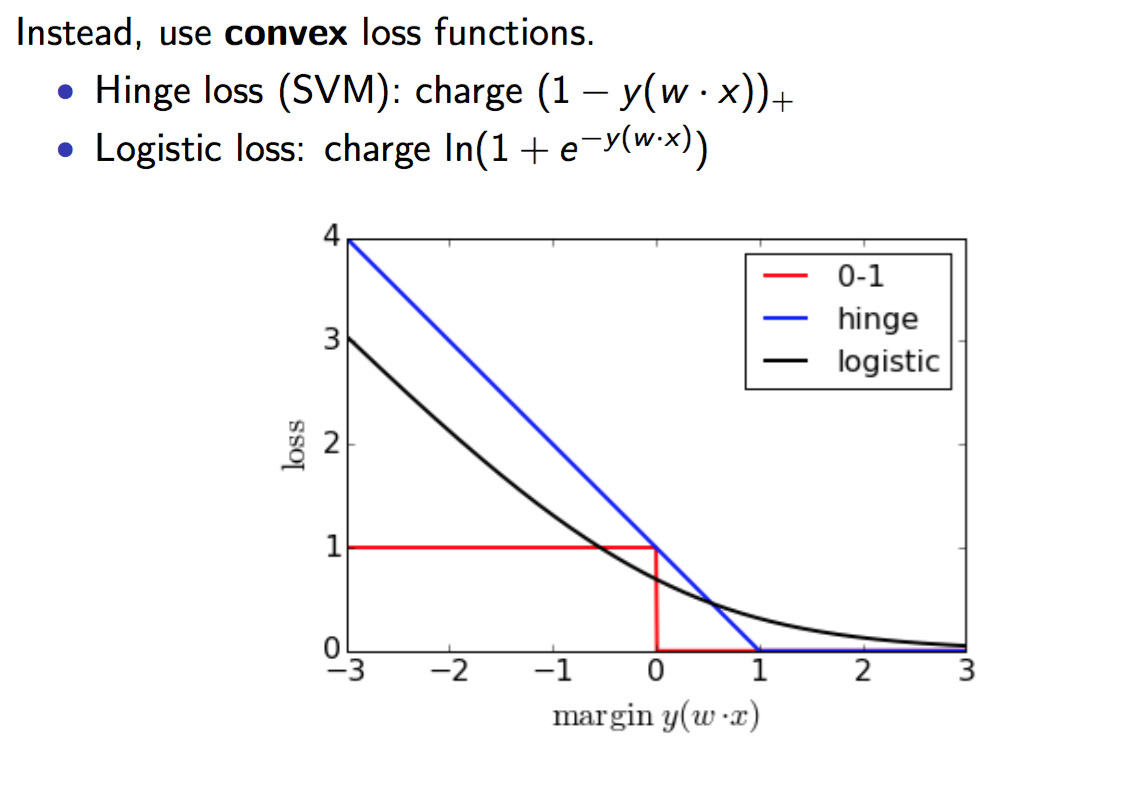
\includegraphics[scale=1.00]{convexSurrogates}}
\caption{Convex Surrogate}
\label{fig:convexSurrogates}
\end{figure}


\chapter{Kernel}
\section{Kernel}
Mapping function $\phi(x)$. 
\section{Kernel Trick}
Weights vector $w$ is a linear combination of $\phi(X): w=A^T\phi(X)$.

Compute $\phi(x)\cdot \phi(x')$, or $<\phi(x), \phi(x')>$, without explicitly compute $\phi(.)$. 

\section{Kernel Functions}
General Form 
\begin{align*}
k(x, x') = \phi(x)\cdot\phi(x')
\end{align*}

Polynomial kernel (high-dim space)
$$
k(x, x')=(1+x\cdot x')^d
$$

String kernel ($+\infty$ dim space: Hilbert space)

\begin{align*}
\phi_s(x)&= s.\text{tf in } x\\
\phi(x) &= (\phi_s(x)|\forall \text{ substring } s). \\
\end{align*}

Gaussian kernel
$$
k(x, x') = \exp\Big(\frac{-||x-x'||^2}{2\sigma^2}\Big)
$$


Kernel matrix: $\{x^{(1)},...,x^{(T)}\}\subset \mat{X}$. 
$$
\mat{K}_{ij} = k(x^{(i)}, x^{(j)}) 
$$

, where $\mat{K}\in \R^{T\times T}$.

Mercer's condition: $\mat{K}$ is PSD.

\chapter{Richer Output Space} 
\section{Multiclass classification}
One weight vector $w_i$ per class. 

\textbf{Predicting.} 
$$
\arg\max_j w_j \cdot x
$$

\textbf{Learning.}
\begin{enumerate}
\item Logistic regression: convex, max data likelihood
$$
\max \prod_i Pr(y^{(i)}|x^{(i)})
$$
\item Perceptron: iterative improvement.

Given a misclassified point $(x, y)$
\begin{align*}
w_y &= w_y + x \\
w_{\hat y} &= w_{\hat y} - x
\end{align*}
\item SVM: convex, min sum of margin with constraints
\begin{align*}
&\min_{w_1, ..., w_k \in \R^p, \xi\in \R^n} \frac{1}{2}\sum_{j=1}^k ||w_j||^2+C\sum_i \xi_i \\
\text{s.t. } &\forall i, \forall y \neq y^{(i)},~ w_{y^{(i)}}\cdot x^{(i)} - w_y \cdot x^{(i)} \geq 1-\xi_i \\
& \forall i,~ \xi_i\geq0
\end{align*}
\end{enumerate}

\section{Structured output spaces}
Single weight vector $w$. 
\begin{enumerate}
\item Feature Vector
$$
\Phi(x, y) = \big(\phi_1(x,y),...,\phi_k(x, y)\big)
$$
\item Predict using linear function of features 
$$
\hat y = \arg\max_y w\cdot \Phi(x, y)
$$
\item Training 
\begin{enumerate}
\item Perceptron
$$
w = w + \Phi(x^{(i)}, y^{(i)})-\Phi(x^{(i)}, \hat y)
$$

\item SVM
\begin{align*}
&\min_{w \in \R^k, \xi\in \R^n} \frac{1}{2}\sum_{j=1}^k ||w||^2+C\sum_i
\xi_i \\
\text{s.t. } &\forall i, \forall y \neq y^{(i)},~  w\cdot \Phi(x^{(i)}, y^{(i)})-w\cdot \Phi(x^{(i)}, y)\geq \Delta(y^{(i)}, y)-\xi_i \\
& \forall i,~ \xi_i\geq0
\end{align*}
\end{enumerate}
\end{enumerate}

\chapter{Boosting, Bagging, Random Forest}
Weighted weak classifier $h_t$

\section{Boosting}
\subsection{Algorithm}
\begin{python}[mathescape]
$D_0(i)=\frac{1}{n}, \forall i$
for t in xrange(T):
  train $h_t: \mat{X}\ra [-1, 1]$ using $D_t$
  calculate margin of success: $r_t=\sum_i D_t(i)y^{(i)}h_t(x^{(i)})\in [-1, 1]$
  calculate strength of update: $\alpha_t = \frac{1}{2}\ln {\frac{1+r_t}{1-r_t}}\in \R$
  reweight distribution: $D_{t+1(i)}\propto D_t(i)\exp\big(-\alpha_t y^{(i)}h_t(x^{(i)})\big)$
  
return $H(x)=sign\Big(\sum_t \alpha_t h_t(x)\Big)$
\end{python}

\subsection{Error Rate}
Training error drop off:
$$
e^{-\gamma^2T/2}
$$

, where $|\sum_i D_t(i)y^{(i)}h_t(x^{(i)})|\geq \gamma$ differs from random by margin $\gamma$.

\subsection{Enhanced Sapce}
Enhanced space: $\forall h \in \mat{H}$ corresponds to a feature 
$$
\phi(x) = \Big(h(x):h\in \mat{H}\Big)
$$

Thus, 
$$
H(x) = sign\Big(\sum_t \alpha_t h_t(x)\Big)
$$

is a linear classifier in the enhanced space $\phi$. 

Boosting is a \textbf{coordinate descent} procedure for minimizing the loss.

\section{Bagging}
Sample with replacement, majority vote.

\section{Random Forest}
Sample $n'$ with replacement, sample $k$ features, majority vote.

\chapter{Clustering}
Representation learning. 

Learn true dof. 

\section{$k$-means}
\subsection{Cost function}
$$
cost(\mu_1, ..., \mu_k) = \sum_{i=1}^n \min_j ||x_i-\mu_j||^2
$$

Sum of distance to the nearest center. 

\subsection{Algorithm}
Lloyd’s $k$-means algorithm

\subsection{Initialization}
\begin{enumerate}
\item Random
\item Extra centers, prune
\item $k$-mean++: iterative add centers to $C$ from data points according to the distribution 
$$
Pr(x) \propto \big(\min_{z\in C}||x-z||\big)^2
$$


\end{enumerate}
\section{EM mixture of Gaussians}
\subsection{Predicting}
$$
Pr(x) = \sum_k \pi_k N(\mu_k, \Sigma_k)
$$

\subsection{Learning}
$$
\max Pr(data|\sum_k \pi_k P_k)
$$

E-step:

calculate the probability of data point $x_i \in cluster~j$. 
\begin{align*}
w_{ij} = Pr(cluster~j|x_i) = \frac{\pi_j P_j(x_i)}{\sum_j \pi_j P_j(x_i)}
\end{align*}

M-step:

M-step for parametric learning 
\begin{align*}
\pi_j &= \frac{1}{n} \sum_{i=1}^n w_{ij} \\
\mu_j &= \frac{1}{n\pi_j} \sum_{i=1}^n w_{ij} x_i \\
\Sigma_j &= \frac{1}{n\pi_j} \sum_{i=1}^n w_{ij}(x_i-\mu_j)(x_i-\mu_j)^T
\end{align*}
\begin{align*}

\end{align*}
\section{Agglomerative hierarchical clustering}
Linkage
\begin{enumerate}
\item Single link
\item Complete link 
\item Average link 
\end{enumerate}


\chapter{Informative Projection}
\section{Projection}
\begin{align*}
x &\in \R^p\\
U^T x &\in \R^k \\
UU^Tx &\in \R^p
\end{align*}

\section{PCA}
$x \mapsto$ a single direction $u$:

The mean is $u^t\mu$
\begin{align*}
\E(u^T X) &= u^T \E(X) \\
&= u^T \mu
\end{align*}

The variance is $u^T \Sigma u$:
\begin{align*}
var(u^T X) &= \E(u^T X-u^T \mu)^2\\
&= \E(u^T(X-\mu))^2\\
&= \E(u^T(X-\mu)(X-\mu)^Tu)\\
&= u^T \E(X-\mu)(X-\mu)^T u  \\
&= u^T \Sigma u
\end{align*}

, where $X-\mu$ is a mat. 

$x \mapsto$ multiple directions:

$$
eigen(\Sigma)
$$

$$
Au = \lambda u
$$

Spectral decomposition. 
$$
M = U\Lambda U^T
$$

, where $U^T$ projects $\vec x$ to M's coordinates, $\Lambda$ scales $\vec x$, and then  $U$ projects back to original coordinates.
\section{Low-Rank Approximation}
\subsection{SVD}
$M$ is not sym. $M\in \R^{p\times q}$
\begin{align*}
M &= U \Lambda V^T \\
M &=UW^T \\
\hat M &=\hat U \hat W^T
\end{align*}

, where $\hat U$ is the first $k$ cols of $U$, $\hat W^T$ is the first $k$ rows of $\hat W$. 

\subsection{Applications}
\subsubsection{Latent semantic indexing (LSI)}
$k$ topics. Topic is latent.

\begin{figure}[!htp]
\centering
\subfloat{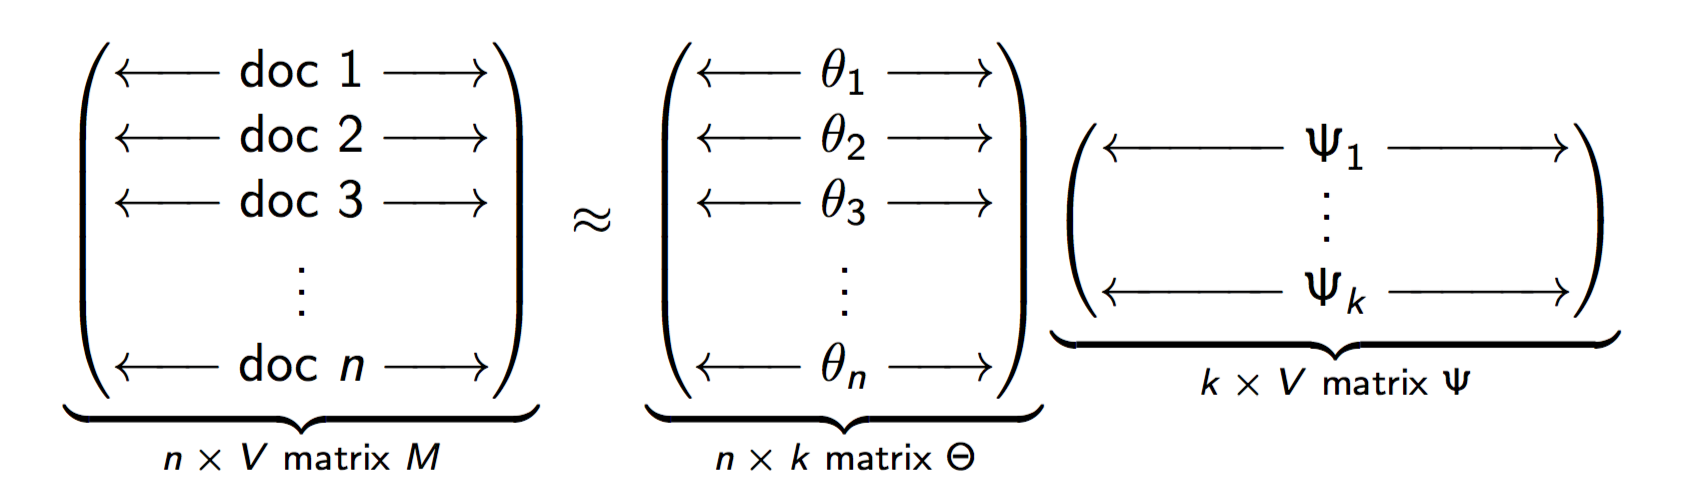
\includegraphics[scale=.80]{lsi}}
\caption{Latent semantic indexing}
\label{fig:lsi}
\end{figure}

What the meanings of $n, V, k$ are.
\subsection{Collaborative filtering}
$k$ latent directions. 

\begin{figure}[!htp]
\centering
\subfloat{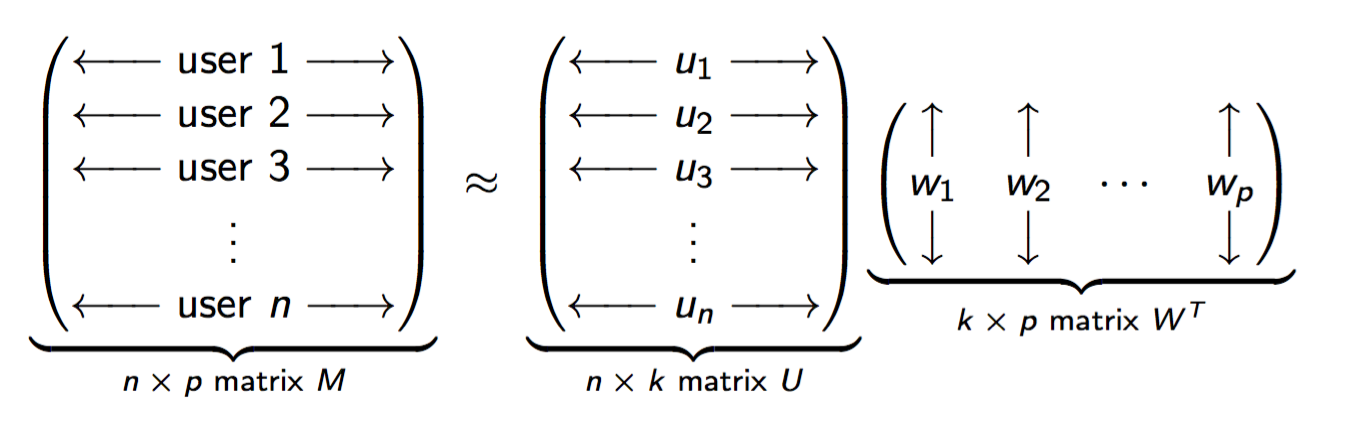
\includegraphics[scale=1.0]{collaborativeFiltering}}
\caption{Collaboraitive Filtering}
\label{fig:collaborativeFiltering}
\end{figure}

What the meanings of $n, p, k$ are. 

\end{document}
